\section{Preface}
This chapter has been submitted to the arXiv preprint server with the following citation: W. M. McFadden, P. M. McCall, and E. M. Munro. Filament turnover is essential for continuous long range contractile flow in a model actomyosin cortex. ArXiv e-prints, December 2016.   \cite{2016arXiv161207430M}


This work was done in collaboration with Patrick McCall in Margaret Gardel's lab and with Edwin Munro at the University of Chicago.  Ed and Patrick directed the outcomes of the project and gave valuable feedback.  Patrick's contributions to the work include careful vetting of both derivations of analytic results and scaling relations derived from the simulations, which uncovered some inconsistencies that I was eventually able to resolve. My contribution was all of the simulation and analysis code.


\section{Introduction}

\paragraph{}  Cortical flow is a fundamental and ubiquitous form of cellular deformation that underlies cell polarization, cell division, cell crawling and multicellular tissue morphogenesis  \cite{cellmech_flows3,cellmech_flows2}.  These flows arise within the actomyosin cortex, a thin layer of cross-linked actin filaments and myosin motors that lies just beneath the plasma membrane   \cite{Salbreux2012536}. The active forces that drive cortical flows are thought to be generated by myosin motors pulling against individual actin filaments   \cite{Munro2004413}. These forces must be integrated within cross-linked networks to build macroscopic contractile stress.  At the same time, cross-linked networks resist deformation and this resistance must be dissipated by network remodeling to allow macroscopic network deformation and flow.  How force production and dissipation depend on motor activity, network architecture and remodeling remains poorly understood.

Current models for cortical flow rely on coarse-grained descriptions of actomyosin networks as active fluids, whose motions are driven by gradients of active contractile stress and opposed by an effectively viscous resistance  \cite{cellmech_flows}.  In these models, gradients of active stress are assumed to reflect spatial variation in motor activity and viscous resistance is assumed to reflect the internal dissipation of elastic resistance due to local remodeling of filaments and/or cross-links   \cite{PhysRevLett.106.028103}.  A key virtue of these models is that their behavior is governed by a few parameters (active stress and effective viscosity).  By coupling an active fluid description to simple kinetic models for network assembly and disassembly and making active stress and effective viscosity depend on e.g network density and turnover rates, it is possible to capture phenomenological descriptions of cortical flow.  Models based on this active fluids description can successfully reproduce spatiotemporal dynamics of cortical flow observed during polarization   \cite{cellmech_flows}, cell division   \cite{Turlier2014114,PhysRevLett.103.058102}, cell motility   \cite{Keren:2009aa,RevModPhys.85.1143} and tissue morphogenesis   \cite{Heisenberg2013948}.  

However, to understand how cells exert physiological control over cortical deformation and flow, or to build and tune networks with desired properties {\em in vitro}, it is essential to connect this coarse-grained description to the microscopic origins of force generation and dissipation within cross-linked actomyosin networks.  Both active stress and effective viscosity depend sensitively on microscopic parameters including densities of filaments, motors and cross-links, force-dependent motor/filament interactions, cross-link dynamics and network turnover rates.  Thus a key challenge is to understand how tuning these microscopic parameters controls the dynamic interplay between active force generation and passive relaxation to control macroscopic dynamics of cortical flow.

\paragraph{} Studies in living cells have documented fluid-like stress relaxation on timescales of 10-100s of seconds   \cite{cellmech_flows,cellmech_flows2,cellmech_flows3,rheo_fluid,rheo_fluid2,cell_rheo_exp}.  These modes of stress relaxation are thought to arise both from the transient binding/unbinding of individual cross-links and from the turnover (assembly/disassembly) of actin filaments.  Studies of cross-linked and/or bundled actin networks {\em in vitro} suggest that cross-link unbinding may be sufficient to support viscous relaxation (creep) on very long timescales  \cite{rheo_crosslinksmatter,rheo_crosslinkslip1,rheo_crosslinkslip2,rheo_crosslinkslip3,rheo_nonaffine}, but is unlikely to explain the rapid large scale cortical deformation and flow observed in living cells.  It has been proposed in the field that rapid actin turnover must play a significant role as well. Indeed, photokinetic and single molecule imaging studies studies reveal rapid turnover of cortical actin filaments in living cells on timescales of 10-100 seconds   \cite{Robin:2014aa}. Previous theoretical models have explored  the dependence of stress relaxation on cross-link binding and unbinding analytically   \cite{theo_crosslinkslip1,theo_crosslinkslip2} and others have explicitly modeled reversible cross-linking in combination with complex mechanics of filament bundles   \cite{model_taeyoon,rheo_crosslinkslip2,theo_crosslinkslip3}, leading to complex viscoelastic stress relaxation.  However, until very recently   \cite{Mak:2016aa} very little attention has been paid to actin turnover as mechanism of stress relaxation. 

Recent work has also begun to reveal insights into mechanisms that govern active stress generation in disordered actomyosin networks. In vitro studies have confirmed that local interactions among actin filaments and myosin motors are sufficient to drive macroscopic contraction of disordered networks   \cite{rheo_2D1}.  Theoretical studies suggest that asymmetrical compliance of actin filaments (stiffer under extension than compression) and spatial differences (dispersion) in motor activity are sufficient conditions for contraction in one   \cite{1367-2630-14-3-033037} and two   \cite{PhysRevX.4.041002} dimensional networks, although other routes to contractility may also exist   \cite{PhysRevX.4.041002}.  Further work has explored how modulation of network architecture, cross-link dynamics and motor density, activity and assembly state can shape rates and patterns of network deformation   \cite{10.1371/journal.pone.0039869,Alvarado:2013aa,C0SM00494D} or network rheology   \cite{0295-5075-85-1-18007,rheo_active}.  

Significantly, {\em in vitro} models for disordered actomyosin networks have used stable actin filaments, and these networks support only transient contraction, either because of network collapse  \cite{Alvarado:2013aa}, or buildup of elastic resistance  \cite{Murrell15062014}, or because network rearrangements (polarity sorting) dissipate the potential to generate contractile force   \cite{Ndlec:1997aa,Surrey1167}. This suggests that continuous turnover of actin filaments may play a key role in allowing sustained deformation and flow. Recent theoretical and modeling studies have begun to explore how this could work   \cite{2015arXiv150706182H,Mak:2016aa,10.1371/journal.pone.0000696}, and to explore dynamic behaviors that can emerge in contractile material with turnover   \cite{PhysRevLett.113.148102}. However, there is much to learn about how the buildup and maintenance of contractile force during continuous deformation and flow depends on the local interplay of network architecture, motor activity and filament turnover.



\paragraph{}  The goal of this work is to build a computational bridge between the microscopic description of cross-linked actomyosin networks and the coarse grained macroscopic description of an active fluid.  We seek to capture the essential microscope features (dynamic cross-links, active motors and semi flexible actin filaments with asymmetric compliance and continuous filament recycling), but in a way that is sufficiently simple to allow systematic exploration of how parameters that govern network deformation and flow in an active fluid theory depend on microscopic parameters. To this end, we introduce several coarse-grained approximations into our representation of filament networks. First, we represent semi-flexible actin filaments as simple springs with asymmetric compliance (stronger in extension than compression). Second, we replace  dynamic binding/unbinding of elastic cross-links with a coarse-grained representation in terms of molecular friction   \cite{theo_friction,theo_frictionSam,theo_molefric}, such that filaments can slide past each other against a constant frictional resistance. Third, we used a similar scheme to introduce active motors at filament crossover points with a simple linear force/velocity relationship, and we introduce dispersion of motor activity by making only a subset of filament overlaps active   \cite{theo_frictionShila}.  Finally, we model filament turnover by allowing entire filaments to appear and disappear with a fixed probabilities per unit time. Importantly, these simplifications allow us to extend our single polymer models to dynamical systems of larger network models for direct comparison between theory and modeling results. This level of coarse graining will therefore make it easier to understand classes of behavior for varying compositions of cross-linked filament networks. In addition, it allows us to compute a new class of numerical simulations efficiently, which gives us concrete predictions for behaviors in widely different networks with measurable dependencies on molecular details. 



\section{Models}


Our motivation is to model essential microscope features of cross-linked actomyosin networks (semi flexible actin filaments with asymmetric compliance, dynamic cross-links, active motors and and continuous filament recycling), in a way that is simple enough to allow systematic exploration of how tuning these microscopic features controls macroscopic network deformation and flow. We focus on 2D networks for computational tractability and because they capture a reasonable approximation of the quasi-2D cortical actomyosin networks that govern flow and deformation in many eukaryotic cells  \cite{cellmech_flows, salbreuxbphs}, or the quasi-2D networks studied recently in vitro  \cite{rheo_2D1,rheo_2D2}.

\begin{figure}[H]
	\centering
	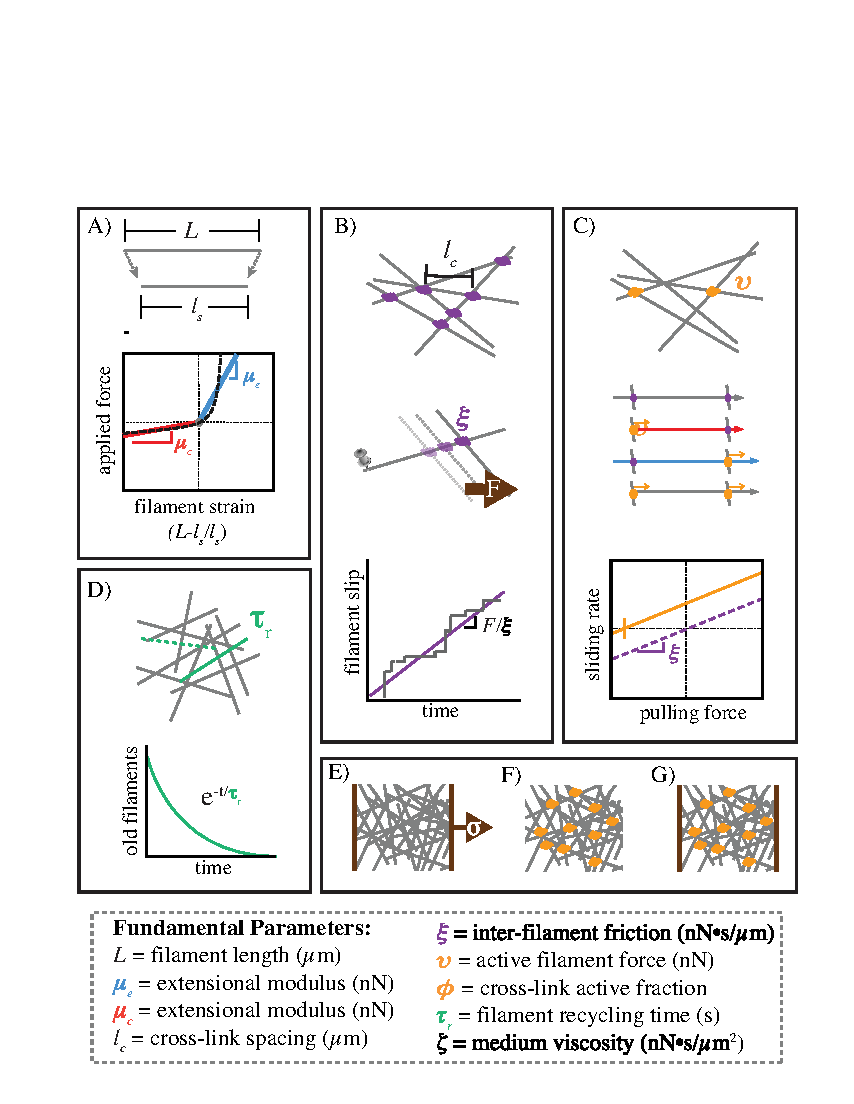
\includegraphics[width=0.8\hsize]{active/figures/Fig1}
	\caption[ Schematic of modeling framework.]{\label{fig:model_overview} Schematic of modeling framework. a) Asymmetric filament compliance.Filaments have smaller spring constant for compression than for extension. b) Cross-link slip. Cross-links are coupled by an effective drag, such that their relative motion is
		proportional to any applied force. c) Motor activity. Filament activity manifests as a basal sliding rate even in the absence of an external force. Only a subset of filament cross-links are active, resulting in differential force exertion along the filament. d) Filament recycling. Filaments are turned over at a constant rate, leading to a refreshing in the strain state of all filaments after a characteristic timescale. e) Applied stress. In simulations with passive cross-links, and external stress is applied as force field acting on a fixed spatial domain.}
\end{figure}

\subsection{Asymmetric filament compliance}
We model individual filaments as chains of springs with relaxed length $l_s$.  Filaments can therefore be represented as a sequence of nodes with positions $\mathbf{x_i}$, where the index $i$ enumerates over all nodes of all segments.  The internal elastic resistance of filament segments gives rise to nearest neighbor force interactions, $\mathbf{F^{\mu}_{i,i+1}}$, of the form

\begin{equation}
\label{eqn:spring}
\mathbf{F^{\mu}_{i,i+1}} = \mu\frac{|\mathbf{x_{i+1}}-\mathbf{x_i}|-l_s}{l_s}\left ( \frac{\mathbf{x_{i+1}}-\mathbf{x_i}}{l_s}\right )
\end{equation}


where the modulus, $\mu$, is a composite quantity representing both filament and cross-linker compliance in a manner similar to a proposed effective medium theory   \cite{theo_crosslinknonlinear}. To model asymmetric filament compliance, we assign a different value to the modulus $\mu$,  depending on whether the strain on a given filament segment, $(|\mathbf{x_{i-1}}-\mathbf{x_i}|-l_s)/l_s$, is greater or less than 0. In the limit of highly rigid cross-links and flexible filaments, our model reduces to the pure semi-flexible filament models of   \cite{theo_hlm,theo_hlm2}. In the opposite regime of nearly rigid filaments and highly flexible cross links, our model is essentially the same as that of   \cite{theo_crosslinknonlinear} in small strain regimes before any nonlinear cross link stiffening. In a departure from those previous models, we assume here that the magnitude of the force on interior cross-links is the same as those on the exterior. This approach ignores the variation in strain on these two sets of cross-links as addressed in   \cite{theo_crosslinknonlinear}, but we choose to ignore this variation in favor of an approximated, global mean approach. 

Because we are dealing with semi-flexible filaments we also introduce a bending modulus between our filament segments such that the restoring force is proportional to the angle between the filament segments and points in the direction orthogonal to the filament direction, $\mathbf{u_i}=(\mathbf{x_{i-1}}-\mathbf{x_{i}})/|\mathbf{x_{i-1}}-\mathbf{x_{i}}|$.   


The total internal force on a filament node i can therefore be written as:

\begin{equation}
\label{eqn:internal}
\mathbf{F^{int}_i} = \mathbf{F^{\mu}_{i-1,i}} + \mathbf{F^{\mu}_{i,i+1}} 
\end{equation}

Introducing a filament bending stiffness adds another mode of asymmetric compliance since filaments can bend/buckle internally under compression. For the majority of the work presented here, we have set $l_s=L$ to obviate dependence on bending driven asymmetries. However, the major points of the paper are still valid for $l_s<L$ under the condition that $\kappa/l_s\gg\mu_c$. 

\subsection{Drag-like coupling between overlapping filaments}
\label{exp_drag}
Previous models represent cross-linkers as elastic connections between pairs of points on neighboring filaments that appear and disappear with either fixed or force-dependent probabilities   \cite{model_taeyoon,theo_crosslinknonlinear}.  Here, we introduce a simpler coarse-grained model for dynamic cross-links by replacing many transient elastic interactions with an effective drag-like coupling between every pair of overlapping segments.
\begin{equation}
\label{eqn:drag}
\mathbf{F^{\xi}_{i-1,i}} = \xi \sum_j \frac{l_s-|s_{ij}-s_i|}{l_s}  (\mathbf{v_{i-1,i}}-\mathbf{v_{j-1,j}}) 
\end{equation}

where $s_i$ is the location (in arc length) of node $i$, $\mathbf{v_{n-1,n}}$ represent the average velocity of the filament segment spanning nodes $n-1$ and $n$, and the sum is taken over all filament segments such that the segment from node $j-1$ to node $j$ intersects the segment from $i-1$ to $i$ at the location $s_{ij}$.

\begin{equation}
\label{eqn:drag}
\mathbf{F^{coup}_{i}} = \mathbf{F^{\xi}_{i-1,i}} + \mathbf{F^{\xi}_{i,i-1}} 
\end{equation}

This model assumes a linear relation between the drag force and the velocity difference between attached segments.  This drag-like coupling has been shown to be an adequate approximation in the case of ionic cross-linking of actin  \cite{mol_fric,theo_hydroish2}, and can be found in the theoretical basis of force-velocity curves for myosin bound filaments  \cite{theo_frictionShila}. Although non-linearities can arise through force dependent detachment kinetics and/or non-linear force extension of cross-links, we assume that inhomogeneities from non-linear effects are of second or higher order. With this assumption, the motion of filaments can be described by a deterministic dynamical equation of the form

\begin{equation}
\label{eqn:syst1}
0 = -l_s\zeta\mathbf{ v_i} -\mathbf{F^{coup}_i}+ \mathbf{F^{int}_i}
\end{equation}

Here, the first term is the filament's intrinsic drag through its embedding fluid, $\zeta$, while the second comes from the drag-like coupling between filaments, $\xi$.  

\subsection{Active coupling for motor driven filament interactions}

To add motor activity we select a subset of cross-linked points and impose an additional force of magnitude $\upsilon$ on each of the overlapping filament segments, directed towards the (+) end of that segment, $\mathbf{u_i}=(\mathbf{x_{i-1}}-\mathbf{x_{i}})/|\mathbf{x_{i-1}}-\mathbf{x_{i}}|$. Thus, the total ``active'' force on a given filament segment is

\begin{equation}
\label{eqn:moto}
\mathbf{F^{\upsilon}_{i-1,i}}=\upsilon \mathbf{u_i}\sum_j \frac{l_s-|s_{ij}-s_i|}{l_s}q_{ij}
\end{equation}

where $q_{ij}$ equals 0 or 1 depending on whether there is an ``active'' cross-linker at this location. To model dispersion of motor activity, we set $q_{ij}=1$  on a randomly selected subset of cross-link points at the beginning of the simulation, such that $\bar{q}=\phi$, where $\bar{q}$ indicates the mean of $q$.  



Finally, for each active force, $\mathbf{F^{act}_j}$, imparted by filament $j$, we must also impart the opposite force onto the filament between $i$ and $i+1$ as well.  Therefore, the entire equation for activity will appear as

\begin{equation}
\label{eqn:active}
\mathbf{F^{act}_{i}}=\mathbf{F^{\upsilon}_{i-1,i}} + \mathbf{F^{\upsilon}_{i,i+1}}
- \sum_{j}\mathbf{F^{\upsilon}_{j-1,j}}q_{ij}
\end{equation}


This will leave us with a full equation of motion given by the sum of each of the parts defined above.

\begin{equation}
\label{eqn:syst3}
0=-L\zeta\mathbf{ v_i} -\mathbf{F^{coup}_i}+ \mathbf{F^{int}_i}+\mathbf{F^{act}_i} 
\end{equation}

\subsection{2D network formation}

We used a mikado model approach   \cite{Unterberger2014} to initialize a minimal network of connected unstressed linear filaments in a rectangular 2D domain. We generate 2D networks of these semi-flexible filaments by laying down straight lines of length, L, with random position and orientation. We then assume that overlapping filaments become cross-linked at their points of overlap. Although real cytoskeletal networks may form with non-negligible anisotropy, for simplicity, we focus on isotropically initialized networks. We define the density using the average distance between cross-links along a filament, $l_c$. A simple geometrical argument can then be used to derive the number of filaments filling a domain as a function of $L$ and $l_c$  \cite{theo_hlm}.  Here, we use the approximation that the number of filaments needed to tile a rectangular domain of size $D_x \times D_y$  is $2D_xD_y/Ll_c$, and that the length density is therefore simply, $2/l_c$. In the absence of cross-link slip, we expect the network to form a connected solid with a well defined elastic modulus  \cite{theo_hlm,theo_hlm2}.


\subsection{External applied stress}
We can model our active networks as a coupled system of differential equations satisfying \ref{eqn:syst3}.  However, to probe the passive response of the network, we also wish to incorporate externally applied stresses.  Although the general passive mechanical response of this system may be very complex, we focus our attention on low frequency deformations and the steady-state creep response of the system to an applied stress.  To do this we introduce a fixed stress, $\sigma$ along a fixed domain at one edge of the network.  The stress is applied via individual forces to the filaments lying within a patch of size $D_w$ such that the sum of individual forces is equal to the applied stress times the height of the domain.  These forces point in the direction, $\mathbf{\hat{x}}$, producing an extension of the patch.  The region of applied stress does not move as the network deforms, allowing us to more easily focus our attention on a fixed sized domain. 

Finally, we add a 0 velocity constraint at the other edge of our domain of interest.  We assume that our network is in the ``dry,'' low Reynold's number limit, where inertial effects are so small that we can equate our total force to 0.  Therefore, we have a dynamical system of wormlike chain filaments satisfying

\begin{equation}
\label{eqn:systfull}
0=-L\zeta\mathbf{ v_i} -\mathbf{F^{coup}_i}+ \mathbf{F^{int}_i}+\mathbf{F^{act}_i} + \sigma\mathbf{\hat{u}(x_i)}
\end{equation}

subject to constraints such that $\mathbf{v_i(x)}$ is 0 with $x=0$.  This results in an implicit differential equation for filament segments which can be integrated in time to produce a solution for the motion of the system.


\subsection{Modeling filament turnover}

In living cells, actin filament assembly is governed by multiple factors that control nucleation, elongation, and filament branching. Likewise filament disassembly is governed by multiple factors that promote filament severing and monomer dissociation at filament ends. Here, we focus on a lowest order model for filament recycling in which entire filaments appear with a fixed rate per unit area, $k_{app}$ and disappear at a rate $k_{diss}\rho$, where $\rho$ is a filament density. With this assumption, in the absence of network deformation, the density of filaments will equilibrate to a steady state density, $k_{app}/k_{diss}$, with time constant $\tau_r = 1/k_{diss}$.   In deforming networks, the density will be set by a competition between strain thinning ($\gamma>0$) or thickening ($\gamma<0$), and density equilibration via turnover. To implement this assumption, at fixed time interval $\tau_s < 0.01\cdot\tau_r$ (i.e. 1\% of the equilibration time), we selected a fraction, $\tau_s/\tau_r$, of existing filaments (i.e. less than 1\% of the total filaments) for degradation. We then generated a fixed number of new unstrained filaments $k_{app}\tau_sD_xD_y$ at random positions and orientations within the original domain.   This method ensures that there is a constant fixed number of filaments present throughout the simulation. We refer to this continuous turnover as filament recycling, to $k_{diss}=1/\tau_r$ as the recycling rate, and to $\tau_r$ as the recycling time.


\subsection{Simulation methods}

Details of our simulation approach and references to our code can be found in the Appendix. Briefly, equations \ref{eqn:spring},\ref{eqn:drag},\ref{eqn:moto} and \ref{eqn:systfull} define a coupled system of ordinary differential equations for the velocities of the endpoints of filament segments, $\mathbf{\dot{x}}$.  These equations are coupled by the effective cross-link friction on segment overlap points, yielding a system of the form:

\begin{equation}
\mathbf{A \cdot \dot x} = \mathbf{f(x)}
\end{equation}

where $\mathbf{A }$ represents a coupling matrix between endpoints of filaments that overlap, and $\mathbf{f(x)}$ is the spring force between pairs of filament segment endpoints.   We numerically integrate this system of equations to find the time evolution of the positions of all filament endpoints. We generate a network of filaments with random positions and orientations as described above within a domain of size $D_x$ by $D_y$.  For all simulations, we imposed periodic boundaries in the y-dimension. When imposing an extensional stress, we constrained all filament segment endpoints within a fixed distance $0.05\cdot D_x$ from the left edge of the domain to be non-moving, then we imposed a rightwards force on all segment endpoints within a distance $0.05\cdot D_x$ from the left edge of the patch.   To simulate free contraction, we removed all constraints at boundaries; to assess buildup of contractile stress under isometric conditions, we used periodic boundary conditions in both $x$ and $y$ dimensions.




We smoothed all filament interactions, force fields, and constraints by allowing forces to decay linearly over small regions such that the equations contained no sharp discontinuities. The nominal units for length, force, and time are $\mu m$, nN, and s, respectively.  We explored parameter space around an estimate of biologically relevant parameter values given in Table \ref{table:para}. 

\begin{table}[h]
	\centering
	\caption{Simulation Parameter Values}
	\label{table:para}
	\begin{tabular}{|c|c|c|c|c|}
		\hline
		{\bf parameter}             & {\bf symbol} & {\bf physiological estimate}          \\ \hline
		extensional modulus         & $\mu_e$        & $1 nN $                                               \\
		compressional modulus             & $\mu_c$     & $ 0.01 nN $                           \\
		cross-link drag coefficient & $\xi$      & $unknown $              \\
		solvent drag coefficient     & $\zeta$        & $0.0005 \frac{nN s}{\mu m^2} $      \\
		filament length             & L            & $5 \mu m$                                          \\
		cross-link spacing          & $l_c$        & $0.5 \mu m$                                         \\
		active filament force          & $\upsilon$        & $0.1 nN$                                         \\
		active cross-link fraction          & $\phi$        & $0.1<0.9$                                         \\
		domain size                 & $D_x\times D_y$            & $20\times 50 \mu m$                                 \\ \hline
	\end{tabular}
\end{table}





\section{Results}
The goal of this study is to understand how cortical flow is shaped by the simultaneous dependencies of active stress and effective viscosity on filament turnover, crosslink drag and on ``network parameters'' that control  filament density, elasticity and motor activity.   We approach this in three steps: First, we analyze the passive deformation of a cross-linked network in response to an externally applied stress; we identify regimes in which the network response is effectively viscous and characterize the dependence of effective viscosity on network parameters and filament turnover.  Second, we analyze the buildup and dissipation of active stress in cross-linked networks with active motors, as they contract against an external resistance; we identify conditions under which the network can produce sustained stress at steady state, and characterize how steady state stress depends on network parameters and filament turnover. Finally, we confirm that the dependencies of active stress and effective viscosity on network parameters and filament turnover are sufficient to predict the dynamics of networks undergoing steady state flow in response to spatial gradients of motor activity.
% PASSIVE SECTION
\subsection{Filament turnover allows and tunes effectively viscous steady state flow.}

% Example of passive simulation measurements
\paragraph{Networks with passive cross-links and no filament turnover undergo three stages of deformation in response to an extensional force.} 

To characterize the passive response of a cross-linked filament network without filament recycling, we simulated a simple uniaxial strain experiment in which we pinned the network at one end, imposed an external stress at the opposite end, and then quantified network strain and internal stress as a function of time (Fig. \ref{fig:model_overview}E). The typical response occurred in three qualitatively distinct phases (Fig. \ref{fig:passive_ex}A,C). At short times the response was viscoelastic, with a rapid buildup of internal stress and a rapid $\sim$exponential approach to a fixed strain (\ref{fig:passive_supp}A), which represents the elastic limit in the absence of cross-link slip predicted by   \cite{theo_hlm}. At intermediate times, the local stress and strain rate were approximately constant across the network (Fig. \ref{fig:passive_ex}B), and the response was effectively viscous; internal stress remained ~constant while the network continued to deform slowly and continuously with nearly constant strain rate (shown as dashed line in Fig. \ref{fig:passive_ex}C) as filaments slip past one another against the effective cross-link drag. In this regime, we can quantify effective viscosity, $\eta_c$,  as the ratio of applied stress to the measured strain rate. Finally, as the network strain approached a critical value ($\sim 30\%$ for the simulation in Fig. \ref{fig:passive_ex}), strain thinning lead to decreased network connectivity, local tearing, and rapid acceleration of the network deformation (see inset in Fig. \ref{fig:passive_ex}C).


\begin{figure}[H]
	\centering
	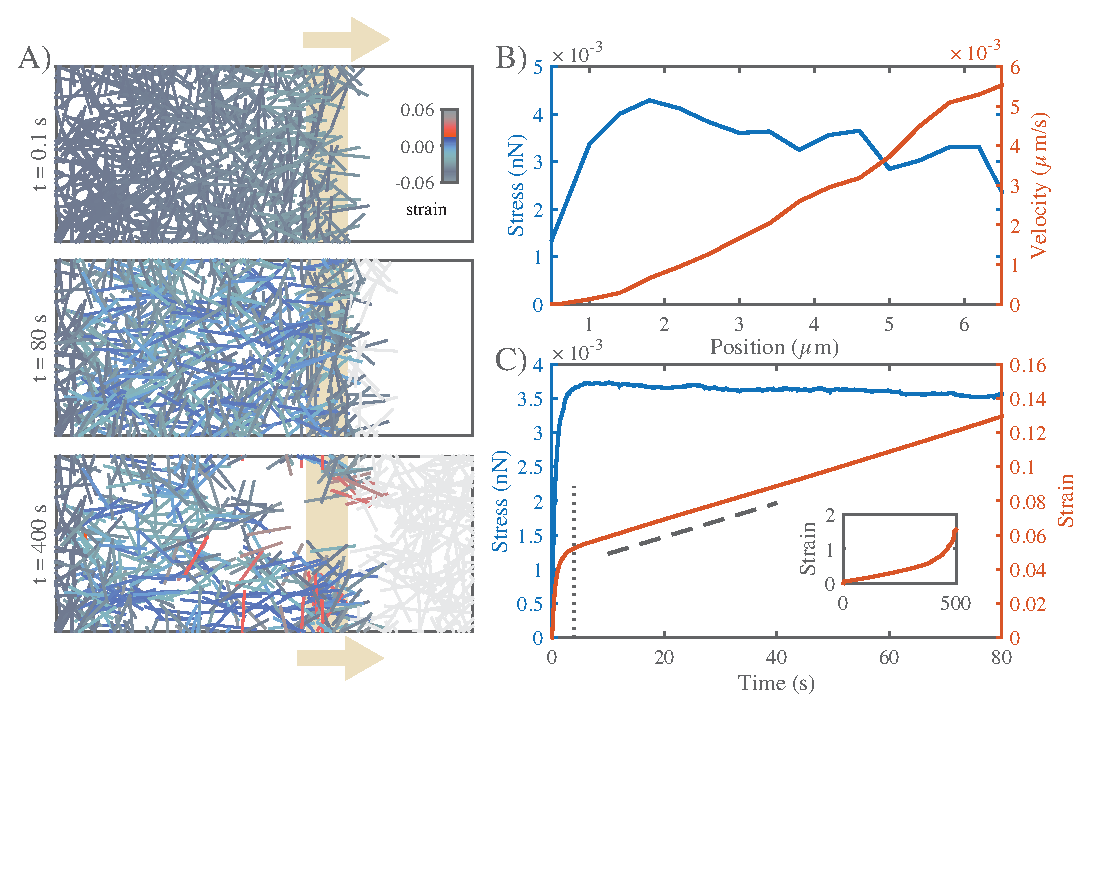
\includegraphics[width=\hsize]{active/figures/Fig2}
	\caption[ Networks with passive cross-links and no filament turnover undergo three stages of deformation in response to an extensional stress.]{\label{fig:passive_ex}  Networks with passive cross-links and no filament turnover undergo three stages of deformation in response to an extensional stress.   \textbf{A)} Three successive time points from a simulation of a $4\times6.6\: \mu m$ network deforming under an applied stress of 0.005 $nN/\mu m$. Stress (tan arrows) is applied to filaments in the region indicated by the tan bar. In this and all subsequent figures, filaments are color-coded with respect to state of strain (blue = tension, red = compression).  Network parameters: $L=1\: \mu m$, $l_c=0.3\: \mu m$, $\xi=100\: nN\cdot s/\mu m$. \textbf{B)} Mean filament stress and velocity profiles for the  network in (a) at t=88s. Note that the stress is nearly constant and the velocity is nearly linear as predicted for a viscous fluid under extension.  \textbf{C)} Plots of the mean stress and strain vs time for the simulation in (a), illustrating the three stages of deformation: (i) A fast initial deformation accompanies rapid buildup of internal network stress; (ii) after a characteristic time $\tau_c$ (indicated by vertical dotted line) the network deforms at a constant rate, i.e. with a constant effective viscosity, $\eta_c$, given by the slope of the dashed line; (iii) at long times, the network undergoes strain thinning and tearing (see inset)}
\end{figure}

% Viscosity and timescale parameter dependence
\paragraph{Network architecture sets the rate and timescales of deformation.}  To characterize how effective viscosity and the timescale for transition to effectively viscous behavior depend on network architecture and cross-link dynamics, we simulated a uniaxial stress test, holding the applied stress constant, while varying filament length $L$, density $l_c$,  elastic modulus $\mu_e$ and cross link drag $\xi$ (see Table \ref{S1_Table}). We measured the elastic modulus, $G_0$, the effective viscosity, $\eta_c$, and the timescale $\tau_c$ for transition from viscoelastic to effectively viscous behavior, and compared these to theoretical predictions. We observed a transition from viscoelastic to effectively viscous deformation for the entire range of parameter values that we sampled.  Our estimate of $G_0$ from simulation agreed well with the closed form solution  $G_0 \sim \mu/l_c$ predicted by a previous theoretical model   \cite{theo_hlm} for networks of semi-flexible filaments with irreversible cross-links (Fig. \ref{fig:passive_form}B). 

\begin{figure}[H]
	\centering
	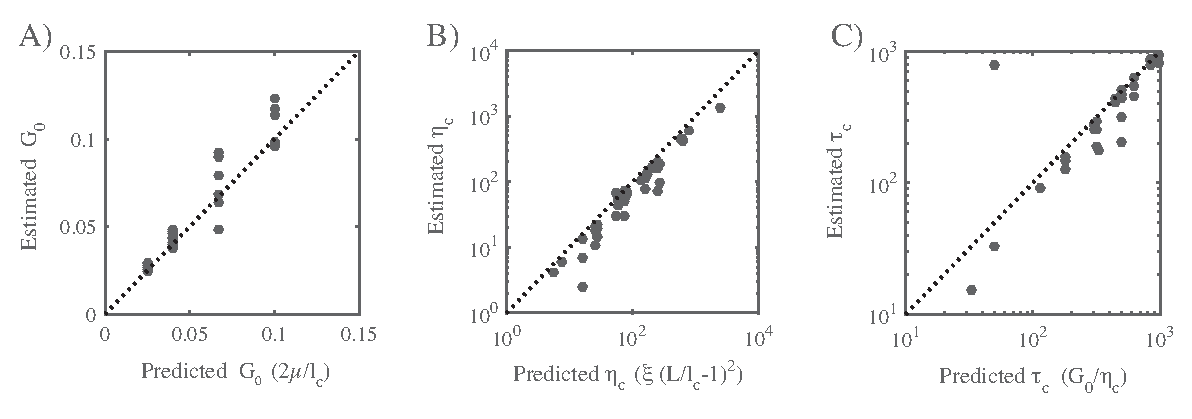
\includegraphics[width=\hsize]{active/figures/Fig3}
	\caption[Network architecture sets the rate and timescales of deformation.]{\label{fig:passive_form} Network architecture sets the rate and timescales of deformation.  \textbf{(a-c)} Comparison of predicted and simulated values for: \textbf{A)} the bulk elastic modulus $G_0$,  \textbf{B)} the effective viscosity $\eta_c$ and \textbf{C)} the timescale for transition from viscoelastic to viscous behavior $\tau_c$, given by the ratio of the bulk elastic modulus $G_0$ to effective viscosity, $\eta_c$. Dotted lines indicates the relationships predicted by theory. }
\end{figure}

A simple theoretical analysis of filament networks with frictional cross link slip, operating in the intermediate viscous regime (see Section \ref{sec:eff_vic}), predicted that the effective viscosity $\eta_c$ should be proportional to the cross-link drag coefficient and to the square of the number of cross-links per filament:

\begin{equation}
	\eta_c = 4\pi\xi\left ( \frac{L}{l_c}-1\right )^2
\end{equation}


As shown in Fig. \ref{fig:passive_form}B, our simulations agree well with this prediction for a large range of sampled network parameters. Finally, for many linear viscoelastic materials, the ratio of effective viscosity to the elastic modulus $\eta_c/G_0$ sets the timescale for transition from elastic to viscous behavior  \cite{mccrum1997principles}. Combining our approximations for $G_0$ and $\eta_c$, we predict a transition time, $\tau_c \approx L^2\xi/l_c\mu$. Measuring the time at which the strain rate became nearly constant (i.e. $\gamma \sim t^n$ with $n>0.8$) yields an estimate of $\tau_c$ that agrees well with this prediction over the entire range of sampled parameters (Fig. \ref{fig:passive_form}C).  Thus the passive response of filament networks with frictional cross link drag is well-described on short (viscoelastic) to intermediate (viscous) timescales by an elastic modulus $G_0$, an effective viscosity $\eta_c$, and a transition timescale $\tau_c$, with well-defined dependencies on network parameters. However, without filament turnover, strain thinning and network tearing limits the extent of viscous deformation to small strains.

% Passive Recycling
\paragraph{Filament turnover allows sustained large-scale viscous flow and defines two distinct flow regimes.} 


To characterize how filament turnover shapes the passive network response to an applied force, we introduced a simple form of turnover in which entire filaments disappear at a rate $k_{diss}\rho$, where $\rho$ is the filament density, and new unstrained filaments appear with a fixed rate per unit area, $k_{app}$. In a non-deforming network,  filament density will equilibrate to a steady state value, $\rho_0 = k_{ass}/k_{diss}$, with time constant $\tau_r = 1/k_{diss}$.  However, in networks deforming under extensional stress, the density will be set by a competition between strain thinning and density equilibration via turnover. 

We simulated a uniaxial stress test for different values of $\tau_r$, while holding all other parameters fixed (Fig. \ref{fig:passive_rec}A-C). For large $\tau_r$, as described above, the network undergoes strain thinning and ultimately tears.  Decreasing $\tau_r$ increases the rate at which the network equilibrates towards a steady state density $\rho_0$.  However, it also increases the rate of deformation and thus the rate of strain thinning (Fig. \ref{fig:passive_rec}B).  We found that the former effect dominates, such that below a critical value $\tau_r = \tau_{crit}$, the network can achieve a steady state characterized by a fixed density and a constant strain rate (\ref{fig:thinning}).  Simple calculations (see Section \ref{sec:couldntbeeasier}) show that the critical value of $\tau_r$ is approximately:

\begin{equation}
	\label{eqn:syst3}
	\tau_{crit} = \frac{\xi {\left (\sqrt{\frac{L}{l_c}}-1 \right )}^3}{\sigma}.
\end{equation}

where  $\sigma$ is the applied stress, $L/l_c$ the linear cross link density, and $\xi$ is the effective crosslink drag. 


\begin{figure}[H]
	\centering
	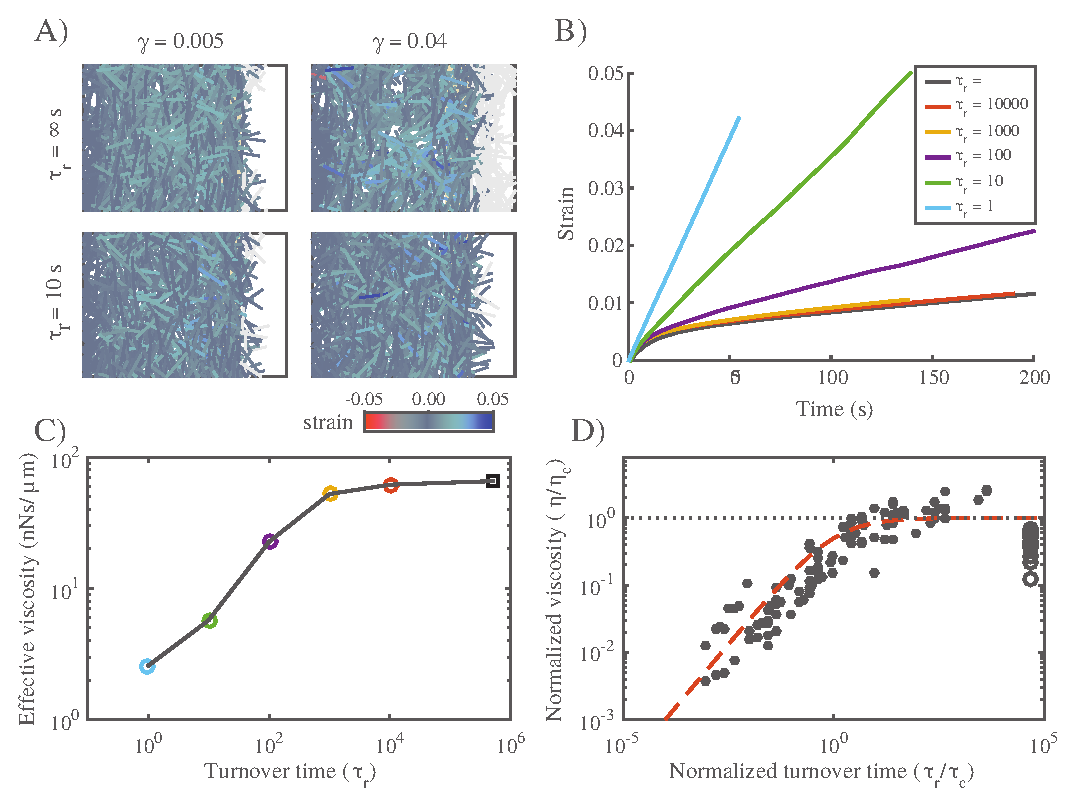
\includegraphics[width=\hsize]{active/figures/Fig4}
	\caption[Filament recycling defines two regimes of effectively viscous flow.]{\label{fig:passive_rec}  Filament recycling defines two regimes of effectively viscous flow. \textbf{A)} Comparison of $20 \times 12 \mu m$ networks under 0.001 $nN/\mu m$ extensional stress without (top) and with (bottom) filament turnover.  Both images are taken when the networks had reached a net strain of 0.04.  For clarity, filaments that leave the domain of applied stress are greyed out. \textbf{B)} Plots of strain vs time for identical networks with different rates of filament turnover.  Network parameters: $L=5\: \mu m$, $l_c=0.5\: \mu m$, $\xi=10\: nN\cdot s/\mu m$. \textbf{C)}  Plot of effective viscosity vs turnover time derived from the simulations shown in panel b.  Square dot is the $\tau_r=\infty$ condition.  \textbf{D)} Plot of normalized effective viscosity ($\eta/\eta_c$) vs normalized turnover time ($\tau_r/\tau_c$) for a large range of network parameters and turnover times. For $tau_r \ll \tau_c$, the viscosity of the network becomes dependent on recycling time. Red dashed line indicates the approximation given in equation \ref{eqn:simple_eta} for $m=3/4$.}
\end{figure}

For $\tau_r < \tau_{crit}$, we observed two distinct steady state flow regimes (Fig. \ref{fig:passive_rec}B,C). For intermediate values of $\tau_r$, effective viscosity remains ~constant with decreasing $\tau_r$.  However, below a certain value of  $\tau_r$ ($\approx 10^3$ for the parameters used in Fig. \ref{fig:passive_rec}C),  effective viscosity decreased monotonically with further decreases in $\tau_r$. To understand what sets the timescale for transition between these two regimes,  we measured effective viscosity at steady steady for a wide range of  network parameters ($L, \mu, {l_c}$), crosslink drags ($\xi$) and filament turnover times (Fig. \ref{fig:passive_rec}D). Strikingly, when we plotted the normalized effective viscosity $\eta_r/\eta_c$ vs a normalized recycling rate $\tau_r/\tau_c$ for all parameter values, the data collapsed onto a single curve, with a transition at  $\tau_r \approx \tau_c$  between an intermediate turnover regime in which effective viscosity is independent of $\tau_r$  and an high turnover regime in which effective viscosity falls monotonically with decreasing $~\tau_r/\tau_c$  (Fig. \ref{fig:passive_rec}D). 

This biphasic dependence of effective viscosity on filament turnover can be understood intuitively as follows:  As new filaments are born, they become progressively stressed as they stretch and reorient under local influence of surrounding filaments, eventually reaching an elastic limit where their contribution to resisting network deformation is determined by effective crosslink drag.  The time to reach this limit is about the same as the time, $\tau_c$, for an entire network of initially unstrained filaments to reach an elastic limit during the initial viscoelastic response to uniaxial stress, as shown in Fig. 2b.  For $\tau_r < \tau_c$, individual filaments do not have time, on average, to reach the elastic limit before turning over; thus the deformation rate is determined by the elastic resistance of partially strained filaments, which increases with lifetime up to $\tau_r = \tau_c$. For $\tau_r > \tau_c$, the deformation rate is largely determined by cross-link resistance to sliding of maximally strained filaments, and the effective viscosity is insensitive to further increase in  $\tau_r$.

These results complement and extend a previous computational study of irreversibly cross-linked networks of treadmilling filaments deforming under extensional stress  \cite{Kim2014526}. Kim et al identified two regimes of effectively viscous deformation: a ``stress-dependent'' regime in which filaments turnover before they become strained to an elastic limit and deformation rate is proportional to both applied stress and turnover rate; and a ``stress-independent'' regime in which filaments reach an elastic limit before turning over and deformation rate depends only on the turnover rate. The fast and intermediate turnover regimes that we observe here correspond to the stress-dependent and independent regimes described by Kim et al, but with a key difference. Without filament turnover, Kim et al's model predicts that a network cannot deform beyond its elastic limit.  In contrast, our model predicts viscous flow at low turnover, governed by an effective viscosity that is set by cross-link density and effective drag. Thus our model provides a self-consistent framework for understanding how crosslink unbinding and filament turnover contribute separately to viscous flow and connects these contributions directly to previous theoretical descriptions of cross-linked networks of semi-flexible filaments. 

In summary, our simulations predict that filament turnover allows networks to undergo viscous deformation indefinitely, without tearing, over a wide range of different effective viscosities and deformation rates. For $\tau_r < \tau_{crit}$, this behavior can be summarized by an equation of the form:

\begin{equation}
	\label{eqn:simple_eta}
	\eta = \frac{\eta_c}{1+(\tau_c/\tau_r)^m}  
\end{equation}

For $\tau_r \gg \tau_c$, $\eta\approx\eta_c$: effective viscosity depends on crosslink density and effective crosslink drag, independent of changes in recycling rate. For $\tau_r\ll\tau_c$,  effective viscosity is governed by the level of elastic stress on network filaments, and becomes strongly dependent on filament lifetime: $\eta\sim\eta_c(\tau_r/\tau_c)^m$. The origins of the $m = 3/4$ scaling remains unclear (see Discussion).




% ACTIVE SECTION
\subsection{Filament turnover allows persistent stress buildup in active networks}

\paragraph{In the absence of filament turnover, active networks with free boundaries contract and then stall against passive resistance to network compression.}


Previous work   \cite{1367-2630-14-3-033037,rheo_2D1,rheo_active} identifies asymmetric filament compliance and spatial heterogeneity in motor activity as minimal requirements for macroscopic contraction of disordered networks. To confirm that our simple implementation of these two requirements (see Models section) is sufficient for macroscopic contraction, we simulated active networks that are unconstrained by external attachments, varying filament length, density, crosslink drag and motor activity.  We observed qualitatively similar results for all choices of parameter values:  Turning on motor activity in an initially unstrained network induced rapid initial contraction, followed by a slower buildup of compressive stress (and strain) on individual filaments, and an $\sim$exponential approach to stall (Fig. \ref{fig:active_con}). The time to stall, $\tau_s$, scaled as $L\xi/\upsilon$ (\ref{fig:active_supp}A). On even longer timescales, polarity sorting of individual filaments, as previously described   \cite{Reymann1310,Murrell15062014,Ndlec:1997aa,Surrey1167} lead to network expansion (see \ref{active_con_video}).


\begin{figure}[H]
	\centering
	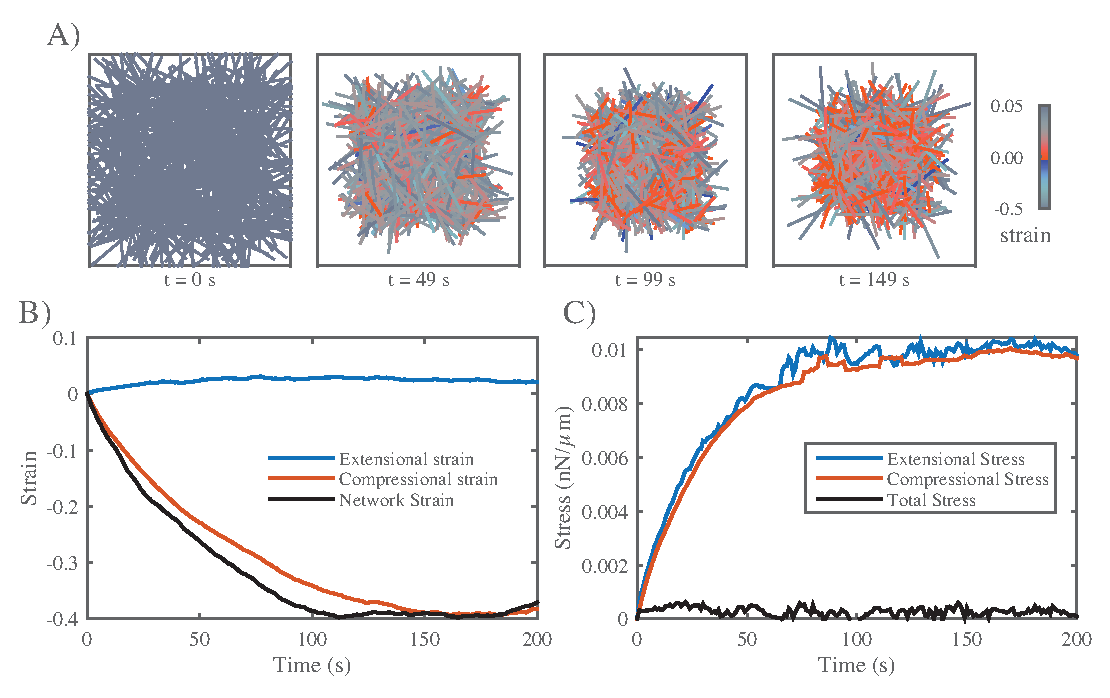
\includegraphics[width=\hsize]{active/figures/Fig5}
	\caption[In the absence of filament turnover, active networks with free boundaries contract and then stall against passive resistance to network compression.]{\label{fig:active_con} In the absence of filament turnover, active networks with free boundaries contract and then stall against passive resistance to network compression. \textbf{A)}  Simulation of an active network with free boundaries. Colors represent strain on individual filaments as in previous figures.  Note the buildup of compressive strain as contraction approaches stall between 100 s and 150 s.  Network parameters: $L=5\: \mu m$, $l_c=0.3\: \mu m$, $\xi=1\: nN\cdot s/\mu m$, $\upsilon=0.1\: nN$.  \textbf{B)} Plots showing time evolution of total network strain (black) and the average extensional (blue) or compressive (red) strain on individual filaments.   \textbf{C)} Plots showing time evolution of total (black) extensional (blue) or compressive (red) stress.  Note that extensional and compressive stress remain balanced as compressive resistance builds during network contraction.}
\end{figure}

During the rapid initial contraction, the increase in network strain closely matched the increase in mean compressive strain on individual filaments Fig. \ref{fig:active_con}B, as predicted theoretically   \cite{1367-2630-14-3-033037,PhysRevX.4.041002} and observed experimentally  \cite{rheo_2D1}. Contraction required asymmetric filament compliance and spatial heterogeneity of motor activity ($\mu_e/\mu_c > 1$, $\phi<1$, \ref{fig:active_supp}B). Thus our model captures a minimal mechanism for bulk contractility in disordered networks through asymmetric filament compliance and dispersion of motor activity. However, in the absence of turnover, contraction is limited by internal buildup of compressive resistance and the dissipative effects of polarity sorting.


\paragraph{Active networks cannot sustain stress against a fixed boundary in the absence of filament turnover.}
\label{pg:explainit}
During cortical flow, regions with high motor activity contract against a passive resistance from neighboring regions with lower motor activity.  To understand how the active stresses that drive cortical flow are shaped by motor activity and network remodeling, we analyzed the buildup and maintenance of contractile stress in active networks contracting against a rigid boundary. We simulated active networks contracting from an initially unstressed state against a fixed boundary (Fig. \ref{fig:active_str}A,B), and  monitored the time evolution of mean extensional (blue), compressional (red) and total (black) stress on network filaments (Fig. \ref{fig:active_str}C,D). We focused initially on the scenario in which there is no, or very slow, filament turnover, sampling a range of parameter values controlling filament length and density, motor activity, and crosslink drag. 

\begin{figure}[H]
	\centering
	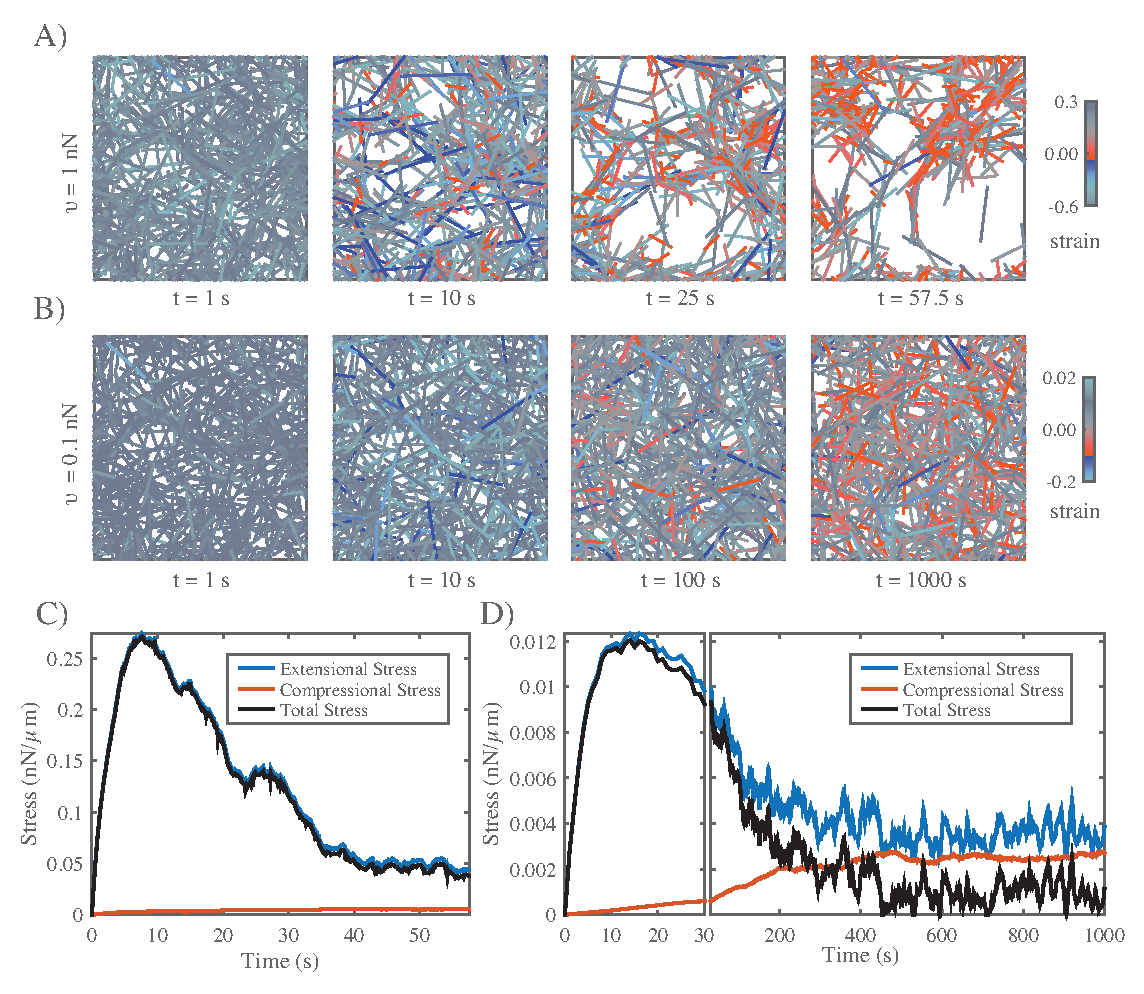
\includegraphics[width=\hsize]{active/figures/Fig6}
	\caption[ In the absence of filament turnover, active networks cannot sustain continuous stress against a fixed boundary.]{\label{fig:active_str} In the absence of filament turnover, active networks cannot sustain continuous stress against a fixed boundary.  \textbf{A)} Simulation of an active network with fixed boundaries. Rearrangement of network filaments by motor activity leads to rapid loss of network connectivity.  Network parameters: $L=5\: \mu m$, $l_c=0.3\: \mu m$, $\xi=1\: nN\cdot s/\mu m$, $\upsilon=1\: nN$.  \textbf{B)} Simulation of the same network, with the same parameter values, except with ten-fold lower motor activity $\upsilon=0.1\: nN$. In this case, connectivity is preserved, but there is a progressive buildup of compressive strain on individual filaments.  \textbf{C)} Plots of total network stress and the average extensional (blue) and compressive (red) stress on individual filaments for the simulation shown in (a). Rapid buildup of extensional stress allows the network transiently to exert force on its boundary, but this force is rapidly dissipated as network connectivity breaks down.  \textbf{D)} Plots of total network stress and the average extensional (blue) and compressive (red) stress on individual filaments for the simulation shown in (b). Rapid buildup of extensional stress allows the network transiently to exert force on its boundary, but this force is dissipated at longer times as decreasing extensional stress and increasing compressive stress approach balance.  Note the different time scales used for plots and subplots in \textbf{C)} and \textbf{D)} to emphasize the similar timescales for force buildup, but very different timescales for force dissipation.}
\end{figure}



We observed a similar behavior in all cases: total stress built rapidly to a peak value $\sigma_m$, and then decayed towards zero (Fig. \ref{fig:active_str}C,D).  The rapid initial increase in total stress was determined largely by the rapid buildup of extensional stress (Fig. \ref{fig:active_str}C,D) on a subset of network filaments (Fig. \ref{fig:active_str}A,B $t=10s$). The subsequent decay involved two different forms of local remodeling: under some conditions, e.g. for higher motor activity (e.g. Fig. \ref{fig:active_str}A,C), the decay was associated with rapid local tearing and fragmentation, leading to global loss of network connectivity as described previously both in simulations  \cite{Mak:2016aa} and {\em in vitro}  experiments   \cite{Alvarado:2013aa}.  However, for many parameters, (e.g. for higher motor activity  as in Fig. \ref{fig:active_str}B,D), the decay in stress occurred with little or no loss of global connectivity.  Instead, local filament rearrangements changed the balance of extensile vs compressive forces along individual filaments, leading to a slow decrease in the average extensional stress, and a correspondingly slow increase in the compressional stress, on individual filaments (see Fig. \ref{fig:active_str}D).  

Combining dimensional analysis with trial and error, we were able to find empirical scaling relationships describing the dependence of maximum stress $\sigma_m$ and the time to reach maximum stress $\tau_m$ on network parameters and effective crosslink drag  ($\sigma_m \sim \sqrt{\mu_e\upsilon}/l_c$, $\tau_m\sim L\xi/\sqrt{\mu_e\upsilon}$, \ref{fig:active_supp}C,D). Although these relationships should be taken with a grain of salt, they are reasonably consistent with our simple intuition that the peak stress should increase with motor force ($\upsilon$), extensional modulus ($\mu_e$) and filament density ($1/l_c$), and the time to reach peak stress should increase with crosslink drag ($\xi$) and decrease with motor force ($\upsilon$) and extensional modulus ($\mu_e$).  

\paragraph{Filament turnover allows active networks to exert sustained stress on a fixed boundary.}

Regardless of the exact scaling dependencies of $\sigma_m$ and $\tau_m$ on network parameters, these results reveal a fundamental limit on the ability of active networks to sustain force against an external resistance in the absence of filament turnover.  To understand how this limit can be overcome by filament turnover, we simulated networks contracting against a fixed boundary from an initially unstressed state, for increasing rates of filament turnover (decreasing $\tau_r$), while holding all other parameter values fixed (Fig. \ref{fig:active_rec}A-C). While the peak stress decreased monotonically with decreasing $\tau_r$, the steady state stress showed a biphasic response, increasing initially with decreasing $\tau_r$, and then falling off as $\tau_r \to 0$.  We observed a biphasic response regardless of how stress decays in the absence of turnover, i.e. whether decay involves loss of network connectivity, or local remodeling without loss of connectivity, or both (\ref{fig:active_tear} and not shown). Significantly, when we plot normalized steady state stress ($\sigma/\sigma_m$) vs normalized recycling time ($\tau_r$/$\tau_m$) for a wide range of network parameters, the data collapse onto a single biphasic response curve, with a peak near $\tau_r/\tau_m = 1$ (Fig. \ref{fig:active_rec}D). In particular, for $\tau_r < \tau_m$, the scaled data collapsed tightly onto a single curve representing a linear increase in steady state stress with increasing $\tau_r$. For $\tau_r > \tau_m$, the scaling was less consistent, although the trend towards a monotonic decrease with increasing $\tau_r$ was clear. These results reveal that filament turnover can rescue the dissipation of active stress during isometric contraction due to network remodeling, and they show that, for a given choice of network parameters, there is an optimal choice of filament lifetime that maximizes steady state stress.

\begin{figure}[H]
	\centering
	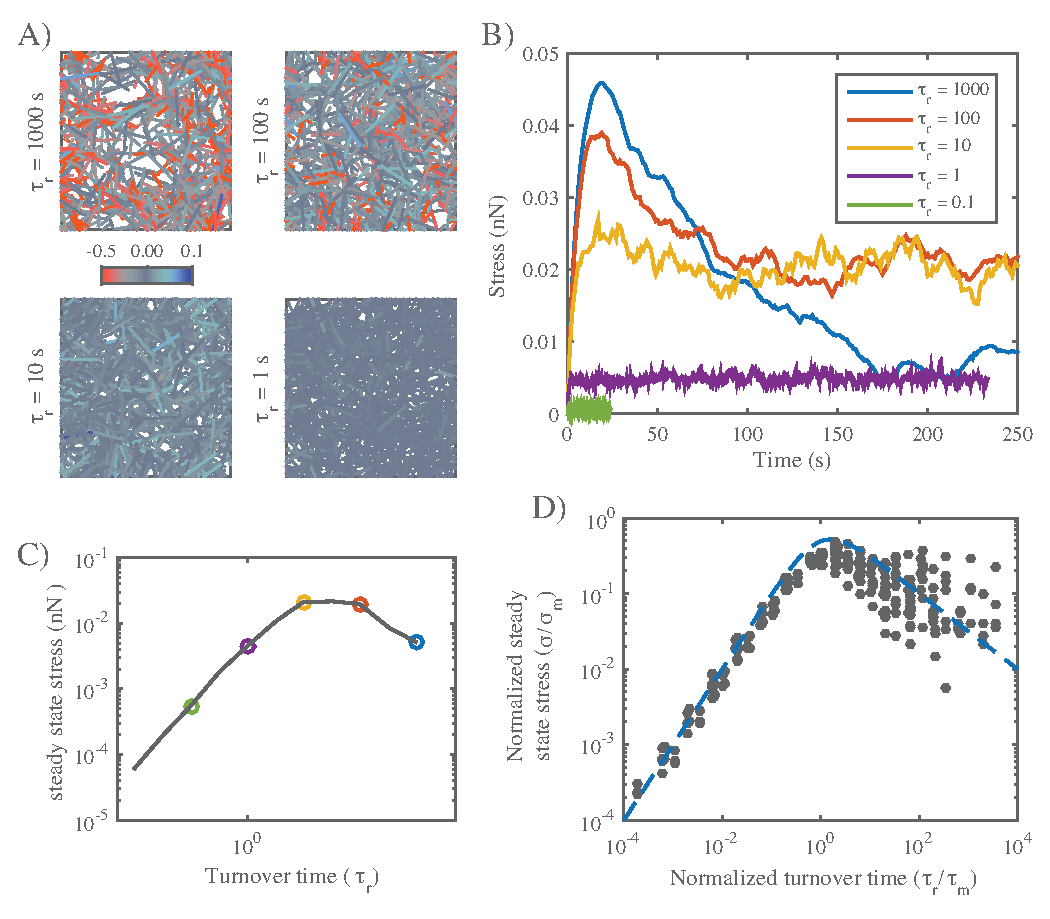
\includegraphics[width=\hsize]{active/figures/Fig7}
	\caption[Filament turnover allows active networks to exert sustained stress on a fixed boundary.]{\label{fig:active_rec} Filament turnover allows active networks to exert sustained stress on a fixed boundary. \textbf{A)} Snapshots from simulations of active networks with fixed boundaries and different rates of filament turnover.  All other parameter values are the same as in Fig. \ref{fig:active_str}A. Note the significant buildup of compressive strain and significant remodeling for longer, but not shorter, turnover times. \textbf{B)} Plots of net stress exerted by the network on its boundaries for different recycling times; for long-lived filaments, stress is built rapidly, but then dissipates. Decreasing filament lifetimes reduces stress dissipation by replacing compressed with uncompressed filaments, allowing higher levels of steady state stress; for very short lifetimes, stress is reduced, because individual filaments do not have time to build stress before turning over. \textbf{C)} Plots of $\approx$steady state stress estimated from the simulations in \textbf{B)} vs turnover time.  \textbf{D)} Plot of normalized steady state stress vs normalized recycling time for a wide range of network parameters and turnover times.  Steady state stress is normalized by the predicted maximum stress $\sigma_{m}$ achieved in the absence of filament turnover.  Turnover time is normalized by the predicted time to achieve maximum stress $\tau_{m}$, in the absence of filament turnover.  Predictions for $\sigma_{m}$ and $\tau_{m}$  were obtained from the phenomenological scaling relations shown in (Fig. \ref{fig:active_supp}C,D). Dashed blue line indicates the approximation given in equation \ref{eqn:simple_sigma} for $n=1$.}
\end{figure}

We can understand the biphasic dependence of steady state stress on filament lifetime using the same reasoning applied to the case of passive flow:   During steady state contraction, the average filament should build and dissipate active stress on approximately the same schedule as an entire network contracting from an initially unstressed state (Fig. \ref{fig:active_rec}B). Therefore for $\tau_r < \tau_m$, increasing lifetime should increase the mean stress contributed by each filament. For $\tau_r > \tau_m$, further increases in lifetime should begin to reduce the mean stress contribution. Directly comparing the time-dependent buildup and dissipation of stress in the absence of turnover, with the dependence of steady state stress on $\tau_r$, supports this interpretation (\ref{fig:recycle_supp})  


As for the passive response (i.e. Equation \ref{eqn:simple_eta}), we can describe this biphasic dependence phenomenologically with an equation of the form:

\begin{equation}
	\label{eqn:simple_sigma}
	\sigma_{ss} = \frac{\sigma_m}{(\tau_r/\tau_m)^n+\tau_m/\tau_r}  
\end{equation}

where the origins of the exponent $n$ remain unclear.




% COMBINED SECTION
\subsection{Filament turnover tunes the balance between active stress buildup and viscous stress relaxation to generate flows}

Thus far, we have considered independently how network remodeling controls the passive response to an external stress, or the steady state stress produced by active contraction against an external resistance. We now consider how these two forms of dependence will combine to shape steady state flow produced by spatial gradients of motor activity. We consider a simple scenario in which a network is pinned on either side and motor activity is continuously patterned such that the right half network has uniformly high levels of motor activity (controlled by $\upsilon$, with $\psi = 0.5$), while the left half network has none. Under these conditions, the right half network will contract continuously against a passive resistance from the left half network.  Because of asymmetric filament compliance, the internal resistance of the right half network to active compression should be negligible compared to the external resistance of the left half network.  Thus the steady state flow will be described by:

\begin{equation}
	\label{eqn:everybody_knows}
	\dot{\gamma} = \frac{\sigma_{ss}}{\eta}  
\end{equation}


where $\sigma_{ss}$ is the active stress generated by the right half-network (less the internal resistance to filament compression), $\eta$ is the effective viscosity of the left half network and strain rate $\dot{\gamma}$ is measured in the left half-network.  Note that strain rate can be related to the steady state flow velocity $v$ at the boundary between right and left halves through $ v = \dot{\gamma}Dx$. Therefore, we can understand the dependence of flow speed on filament turnover and other parameters using the approximate relationships summarized by equations \ref{eqn:simple_eta} and \ref{eqn:simple_sigma} for $\eta$ and $\sigma_{ss}$.  As shown in Fig. \ref{fig:flow_theo}, there are two qualitatively distinct possibilities for the dependence of strain rate on $\tau_r$, depending on the relative magnitudes of $\tau_m$ and $\tau_c$.  In both cases, for fast enough turnover ($\tau_r < \min \left (\tau_m, \tau_c \right )$), we expect weak dependence of strain rate on $\tau_r$ ($ \dot{\gamma}\sim \tau_r^{1/4}$).  For all parameter values that we sampled in this study (which were chosen to lie in a physiological range), $\tau_m > \tau_c$. Therefore we predict the dependence of steady state strain rate on $\tau_r$ shown in Fig. \ref{fig:flow_theo}A.


\begin{figure}[H]
	\centering
	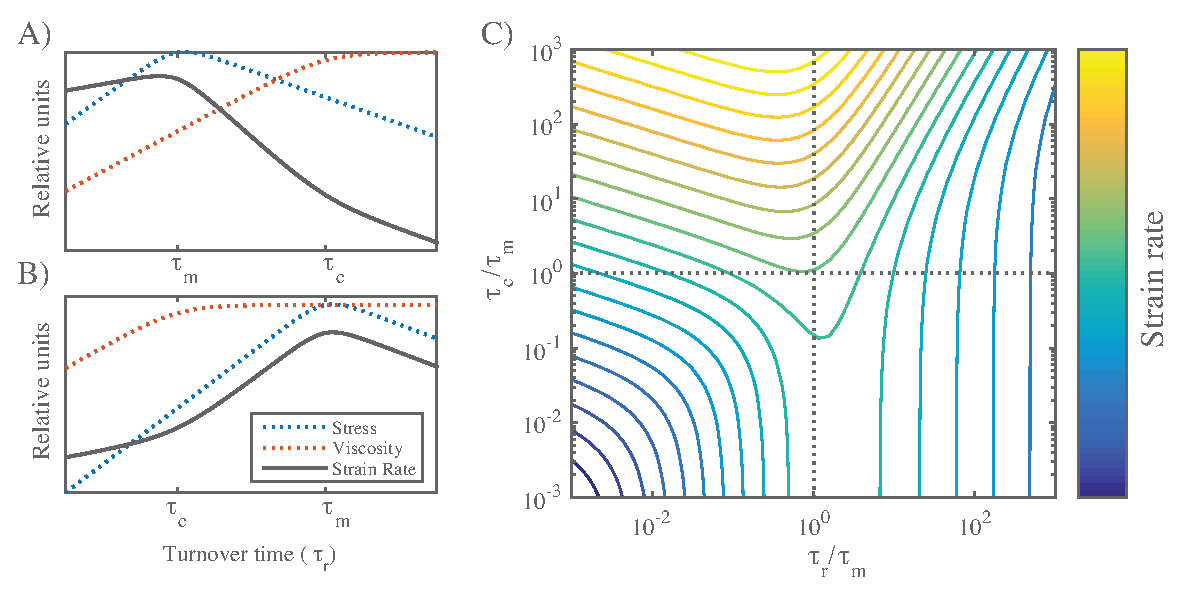
\includegraphics[width=\hsize]{active/figures/Fig8}
	\caption[ Filament recycling tunes the magnitudes of both effective viscosity and steady state stress.]{\label{fig:flow_theo}  Filament recycling tunes the magnitudes of both effective viscosity and steady state stress. \textbf{A)}  Dependence of steady state stress, effective viscosity, and resulting strain rate on recycling time $\tau_r$ under the condition $\tau_{m}<\tau_c$. \textbf{B)} Same as a) but for $\tau_c<\tau_{m}$.  \textbf{C)} State space of flow rate dependence relative to the two relaxation timescales, $\tau_r$ and $\tau_c$ normalized by the stress buildup timescale, $\tau_{m}$.  }
\end{figure}

To confirm this prediction, we simulated the simple scenario described above for a range of values of $\tau_r$, with all other parameter values initially fixed. As expected, we observed a sharp dependence of steady state flow speeds on filament recycling rate (Fig. \ref{fig:flow_ex}B,C). For very long recycling times, ($\tau_r=1000 s$, dark blue line), there was a rapid initial deformation (contraction of the active domain and dilation of the passive domain), followed by a slow approach to a steady state flow characterized by slow contraction of the right half-domain and a matching dilation of the left half-domain (see \ref{fig:combo_prof}).  However, with decreasing values of $\tau_r$, steady state flow speeds increased steadily, before reaching an approximate plateau on which flow speeds varied by less than 15 \% over more than two decades of variation in $\tau_r$ (Fig. \ref{fig:flow_ex}C).  

\begin{figure}[H]
	\centering
	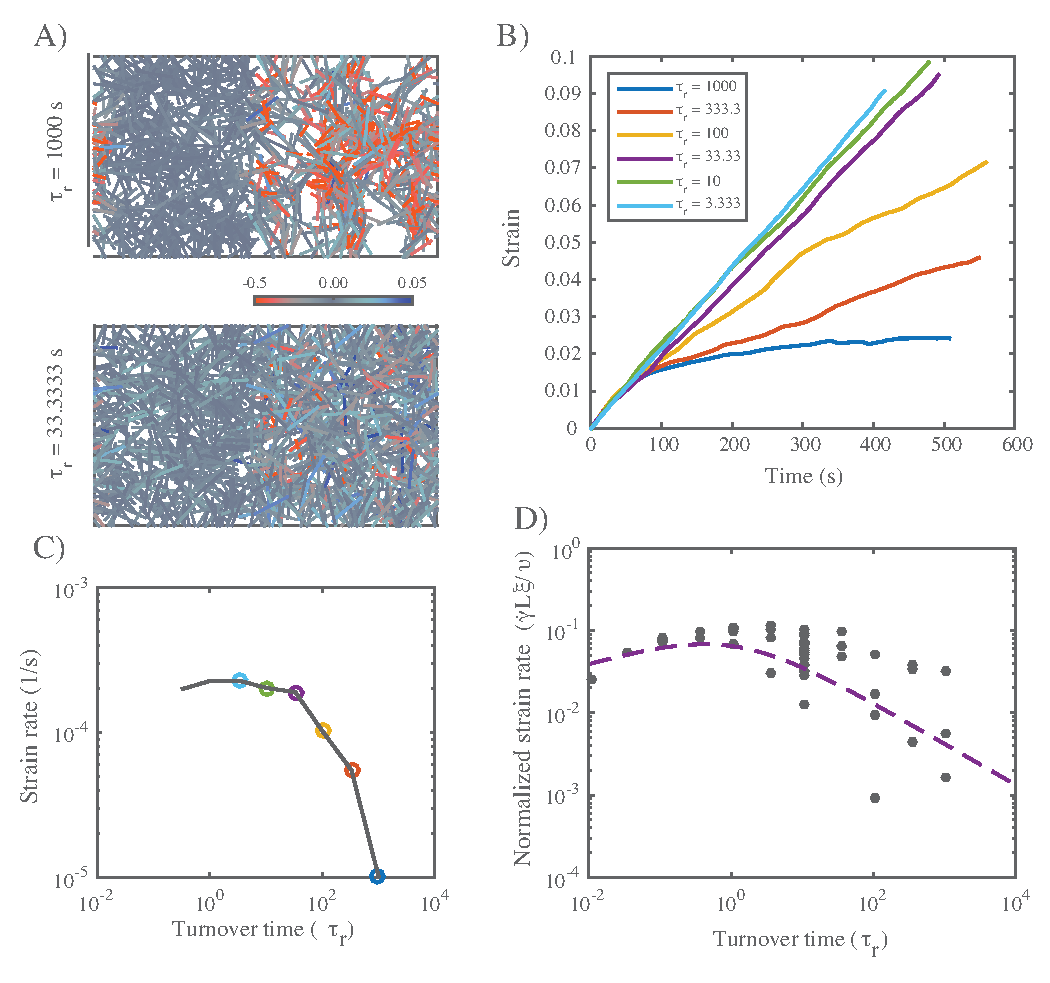
\includegraphics[width=\hsize]{active/figures/Fig9}
	\caption[Filament recycling allows sustained flows in networks with non-isotropic activity.]{\label{fig:flow_ex}  Filament recycling allows sustained flows in networks with non-isotropic activity. \textbf{A)} Example simulations of non-isotropic networks with long ($\tau_r=1000$) and short ($\tau_r=33$) recycling timescales. In these networks the left half of the network is passive while the right half is active.  Network parameters are same as in Fig.s \ref{fig:active_str} and \ref{fig:active_rec}. Importantly, in all simulations $\tau_{m}<\tau_c$. \textbf{B)} Graph of strain for identical networks with varying recycling timescales.  With long recycling times, the network stalls; reducing the recycling timescale allows the network to persist in its deformation.  However, for the shortest recycling timescales, the steady state strain begins to slowly return to 0 net motion.  Measurements are based on the passive side of the network. \textbf{C)} Steady state strain rates for the networks in (b).     \textbf{D)} Graph of network's long-term strain rate as a function of recycling timescale. Dashed line is form of dependence predicted by the  theoretical arguments shown in Fig. \ref{fig:flow_theo}.}
\end{figure}

We repeated these simulations for a wider range of parameter values, and saw similar dependence of $\dot{\gamma}$ on $\tau_r$ in all cases.  Using equation \ref{eqn:simple_eta} with $\tau_r < \tau_c$ and equation \ref{eqn:simple_sigma} with $\tau_r < \tau_m$, and the theoretical or empirical scaling relationships found above for $\eta_c$, $\tau_c$, $\sigma_m$ and $\tau_m$, we predict a simple scaling relationship for $\dot{\gamma}$ (for small $\tau_r$):


\begin{equation}
	\label{eqn:flow_scaling_eq}
	\dot{\gamma} = \frac{\upsilon}{\xi L}  \left ( \tau_r \right ) ^{1/4}
\end{equation}

Indeed, when we plot the steady state measurements of $\dot{\gamma}$, normalized by $\upsilon/\xi L$,  for all parameter values, the data collapse onto a single curve for small $\tau_r$.  Thus. our simulations identify a flow regime, characterized by sufficiently fast filament turnover, in which the steady state flow speed is buffered against variation in turnover, and has a relatively simple dependence on other network parameters.



%Conclusion
\section{Discussion}

\paragraph{} Cortical flows arise through a dynamic interplay of force production and dissipation within cross-linked actomyosin networks. Here we combined computer simulations with simple theoretical analysis to explore how this interplay depends on motor activity, crosslink dynamics, network architecture and filament turnover. Our results reveal two essential requirements for filament turnover during cortical flow:  (a) to allow the continuous relaxation of elastic resistance without catastrophic loss of network connectivity and (b) to prevent the dissipation of active stress through local network rearrangements. We find that biphasic dependencies of active stress and passive relaxation on filament lifetime define multiple modes of steady state flow with distinct dependencies on network parameters and filament turnover.


\paragraph{} We identify two distinct modes of passive response to uniaxial stress:  a low turnover mode in which filaments strain to an elastic limit before turning over, and effective viscosity depends on crosslink density and effective crosslink friction, and a high turnover mode in which filaments turn over before reaching an elastic limit and effective viscosity is proportional to elastic resistance and $\approx$ proportional to filament lifetime. We note that the weakly sub-linear dependence of effective viscosity on filament lifetime that we observe in the high turnover regime may simply reflect a failure to capture very local modes of filament deformation, since a previous study   \cite{Kim2014526} in which filaments were represented as connected chains of smaller segments predicted linear dependence of effective viscosity on filament lifetime. While previous studies have emphasized individual roles for cross-link unbinding or filament turnover in stress relaxation   \cite{De-La-Cruz:2015aa,De-La-Cruz:2009aa,Salbreux2012536}, here we have capture their distinct contributions within a single self-consistent modeling framework. 

\paragraph{} Our simulations confirm the theoretical prediction   \cite{1367-2630-14-3-033037,rheo_2D1,rheo_active} that spatial heterogeneity of motor activity and asymmetric filament compliance are sufficient to support macroscopic contraction of unconstrained networks. However, under isometric conditions, and without filament turnover, our simulations predict that active stress cannot be sustained. On short timescales, motor forces drive local buildup of extensional stress, but on longer timescales, active local filament rearrangements drive local changes in connectivity that lead, invariably, to a decay in active stress.  Under some conditions, contractile forces drive networks towards a critically connected state, leading to tearing and fragmentation, as previously described   \cite{Alvarado:2013aa, Mak:2016aa}. However, we find that stress decay can also occur without any global loss of connectivity, through a gradual decrease in extensile force and a gradual increase in compressive force along individual filaments.   Our results suggest that when filaments can slide relative to one another, the motor forces that produce active stress will inevitably lead to local changes in connectivity that decrease active stress.  Thus for contractile networks to maintain isometric tension on long timescales, they must either form stable crosslinks to prevent filament rearrangements, or they must continuously recycle network filaments (or active motors) to renew the local potential for production of active stress.

\paragraph{} Indeed, our simulations predict that filament turnover is sufficient for maintenance of active stress. As in the passive case, they predict biphasic dependence of steady state stress on filament turnover: For short-lived filaments ($\tau_r < \tau_m$), steady state stress increases linearly with filament lifetime because filaments have more time to build towards peak extensional stress before turning over.  For longer lived filaments ($\tau_r > \tau_m$), steady state stress decreases monotonically with filament lifetime because local rearrangements decrease the mean contributions of longer lived filaments. These findings imply that for cortical networks that sustain contractile stress under approximately isometric conditions, tuning filament turnover can control the level of active stress, and there will be an optimal turnover rate that maximizes the stress, all other things equal.  This may be important, for example in early development, where contractile forces produced by cortical actomyosin networks maintain, or drive slow changes in, cell shape and tissue geometry   \cite{Salbreux2012536,Gorfinkiel2011531}.


\paragraph{} For cortical networks that undergo steady state flows driven by spatial gradients of motor activity, our simulations predict that the biphasic dependencies of steady state stress and effective viscosity on filament lifetime define multiple regimes of steady state flow, characterized by different dependencies on filament turnover (and other network parameters).  In particular, the $\sim$linear dependencies of steady state stress and effective viscosity on filament lifetime for short-lived filaments define a fast turnover regime in which steady state flow speeds are buffered against variations in filament lifetime, and are predicted to depend in a simple way on motor activity and crosslink resistance.  Measurements of F-actin turnover times in cells that undergo cortical flow   \cite{Theriot1991,Murthy2016,Watanabe1083,Guha2016,Fritzsche15032013,Robin:2014aa} suggests that they may indeed operate in this fast turnover regime, and recent studies in {\em C. elegans} embryos suggests that cortical flow speeds are surprisingly insensitive to depletion of factors (ADF/Cofilin) that govern filament turnover   \cite{cellmech_flows}, consistent with our model's predictions. Stronger tests of our model's predictions will require more systematic analyses of how flow speeds vary with filament and crosslink densities, motor activities, and filament lifetimes.



\paragraph{S1 Video.}
\label{passive_ex_video}
{\bf Extensional strain in passive networks.}  Movie of simulation setup shown in Fig. \ref{fig:passive_ex}.  Colors are the same as in figure.

\paragraph{S2 Video.}
\label{active_con_video}
{\bf Active networks contracting with free boundaries.}  Movie of simulation setup shown in Fig. \ref{fig:active_con}.  Colors are the same as in figure.